\section{Lasttest}
Der Lasttest simuliert eine realistische Nutzungslast auf dem System.
Jeder parallele Prozess führt dabei einen vollständigen Ablauf durch:
Login als Mitarbeiter, Rückgabe eines Buches und anschließender Logout.
Jeder Mitarbeiter arbeitet mit einem eigenen Mitglied und Barcode,
um Konflikte zu vermeiden. Die Gesamtdauer wird in Millisekunden gemessen
und zusammen mit der Anzahl erfolgreicher und fehlgeschlagener Anfragen
in einer CSV-Datei gespeichert. 
\begin{figure}[H]
     \centering
     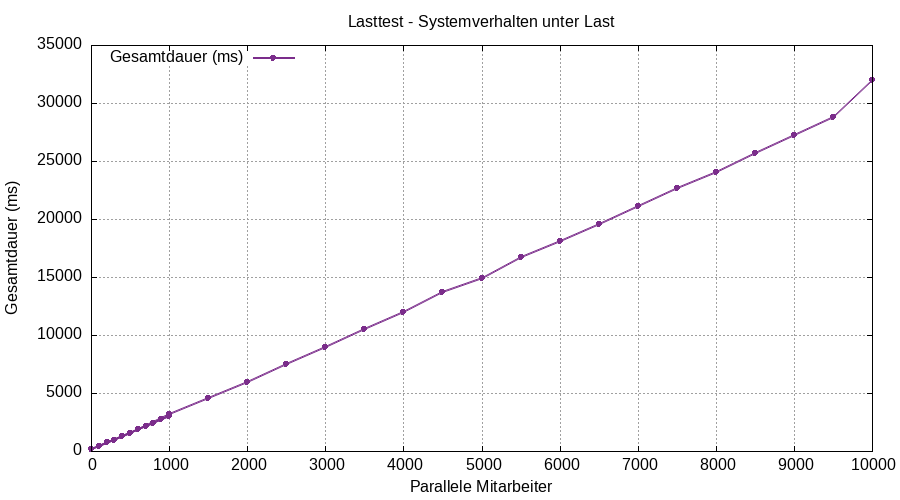
\includegraphics[width=1\linewidth]{src/abbildungen/lasttest.png}
     \caption{Lasttest}
   \end{figure}

   Eine nahezu lineare Kurve zeigt, dass die Infrastruktur (Tomcat, DB-Verbindungspool) auch unter steigender Last stabil und ohne Sättigung skaliert.
